\section {Wiktoria Kowalska}
Wyrażenie matematyczne: 
\[(a+b)(a-b)=a^2-b^2\]

\begin{figure} [htbp]
    \centering
    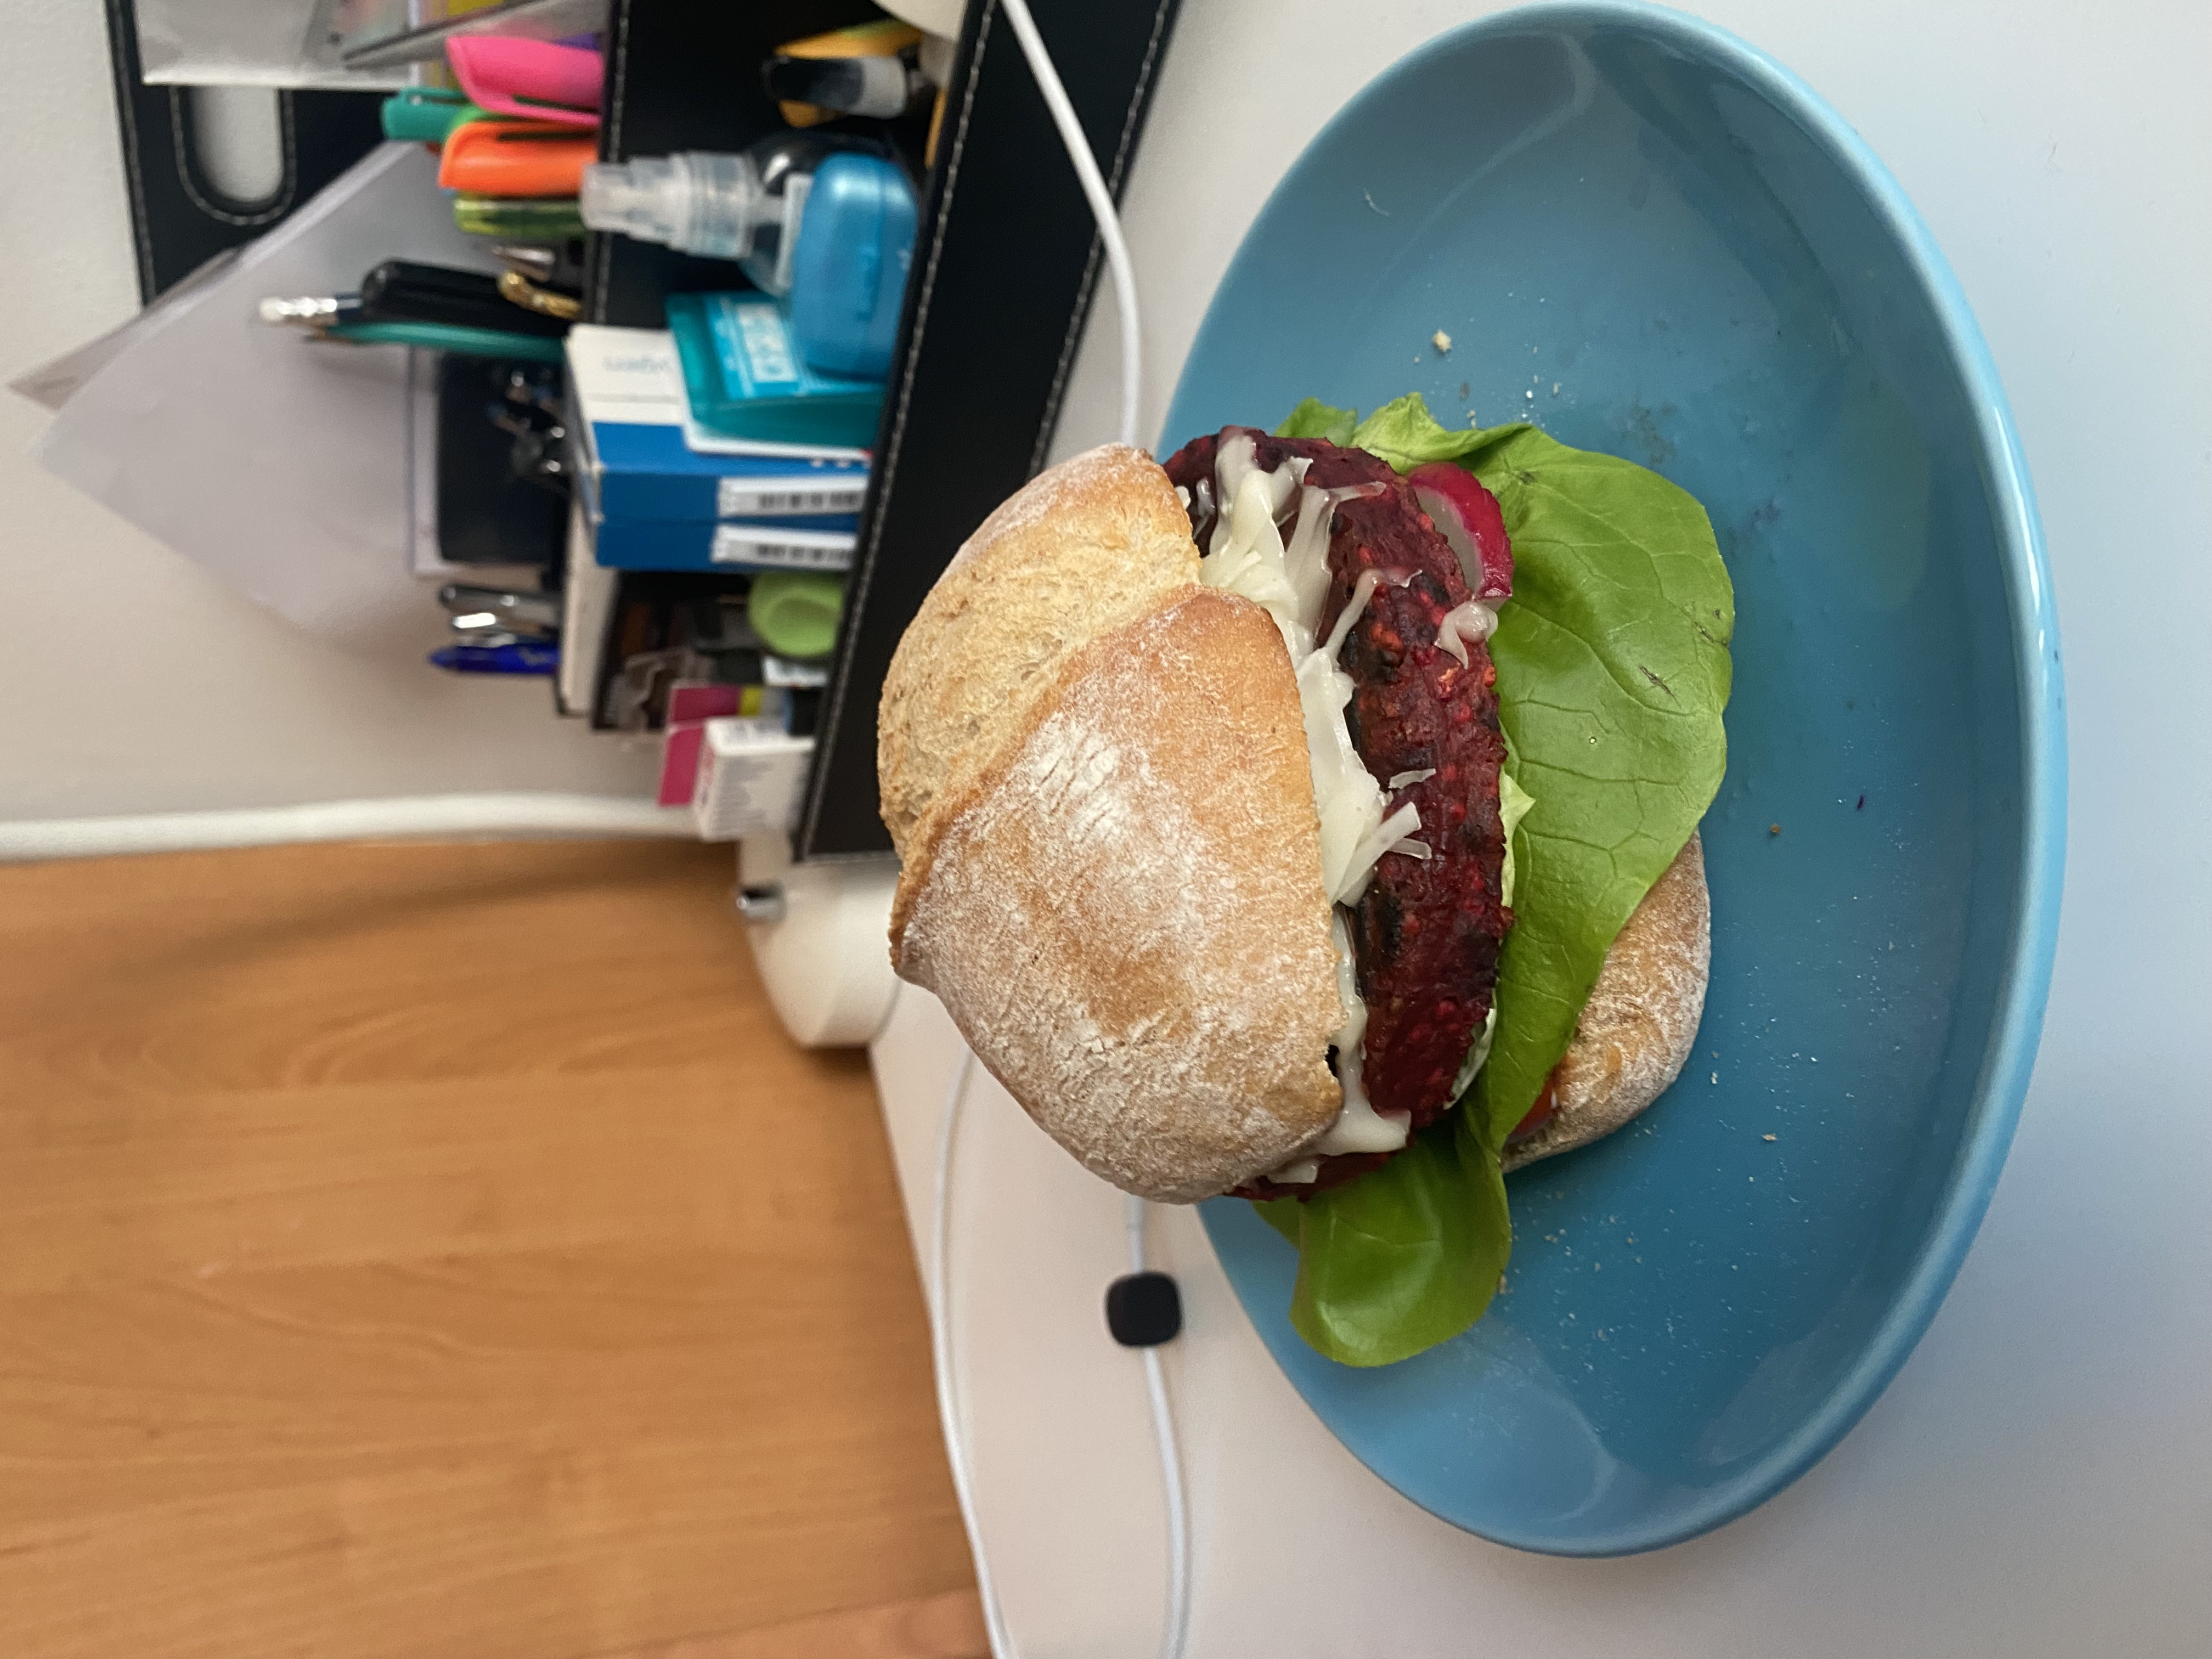
\includegraphics[angle=270,scale=0.05]{pictures/burgerek.jpeg}
    \caption{Mój dzisiejszy obiad}
\end{figure}

Tabelka
\begin{table}[htbp]
    \centering
\begin{tabular}{|l|l|l|l|}
\hline
  & A  & B  & 0 \\ \hline
A & A  & AB & A \\ \hline
B & AB & B  & B \\ \hline
0 & A  & B  & 0 \\ \hline
\end{tabular}
\caption{Grupy}
\label{tab:tabela4}
\end{table}
\\


Lista numerowana:
\begin{enumerate}
    \item uno
    \item dos
    \item tres
\end{enumerate}


Lista nienumerowana:
\begin{itemize}
    \item śniadanie
    \item obiad
    \item kolacja
\end{itemize}


\textbf{Rowing}, sometimes called crew in the United States, is the sport of racing boats using oars. It differs from paddling sports in that rowing oars are attached to the boat using oarlocks, while paddles are not connected to the boat. Rowing is divided into two disciplines: sculling and sweep rowing. In sculling, each rower holds two oars—one in each hand, while in sweep rowing each rower holds one oar with both hands. There are several boat classes in which athletes may compete, ranging from single sculls, occupied by one person, to shells with eight rowers and a coxswain, called eights. There are a wide variety of course types and formats of racing, but most elite and championship level racing is conducted on calm water courses 2 kilometres (1.2 mi) long with several lanes marked using buoys.

\textit{Modern rowing} as a competitive sport can be traced to the early 17th century when professional watermen held races (regattas) on the River Thames in London, England. Often prizes were offered by the London Guilds and Livery Companies. Amateur competition began towards the end of the 18th century with the arrival of "boat clubs" at British public schools. Similarly, clubs were formed at colleges within Oxford and Cambridge in the early nineteenth century. Public rowing clubs were beginning at the same time in England, Germany, the United States. In 1843, the first American college rowing club was formed at Yale College.